\documentclass[12pt,a4paper]{article}
\usepackage[utf8]{inputenc}
\usepackage[ngerman]{babel}
\usepackage{amsmath}
\usepackage{graphicx}
\usepackage{geometry}
\geometry{verbose,a4paper,tmargin=25mm,bmargin=25mm,lmargin=20mm,rmargin=20mm}
\renewcommand{\theequation}{\arabic{section}.\arabic{equation}}
\usepackage{amsfonts}
\usepackage{amssymb}
\usepackage{amsthm}
\usepackage{mathpazo}
\usepackage{subfigure}
\usepackage{hyperref}
\usepackage{enumitem}
\usepackage{multirow}
\usepackage{pdfpages}
\usepackage{wrapfig}
\usepackage{rotating}
\setlength{\parindent}{0pt}
\usepackage{scrpage2}


%Beacause the other chreisli are awful
\def \chreisli[#1]{\raisebox{.5pt}{\textcircled{\raisebox{-.9pt} {#1}}}}

\setcounter{tocdepth}{2} 
\begin{document}


\begin{center}


\newcommand{\HRule}{\rule{\linewidth}{0.5mm}}

{\begin{Huge}\textbf{P3T7}\end{Huge}}
\HRule \\[0.5cm]

\begin{tabular}{l l}
\textbf{Auftraggeber:} & Hans Gysin \\[0.2cm]
\textbf{Betreuende Dozenten:} & Pascal Schleuniger  \\ & Matthias Meier \\  & Anita Gertiser \\& Bonnie Domenghino \\[0.2cm]
\textbf{Projektteam:} & Benjamin Ebeling, Projektleiter \\ & Elias von Däniken \\ & Marc de Bever \\ & Dominik Hiltbrunner   \\[0.2cm]
\textbf{Studiengang:} & Elektro- und Informationstechnik\\\

\end{tabular}
\begin{tabular}{l l}
\HRule \\[0.5cm]
\end{tabular}
\end{center}



\section{Funktionsprinzip}
In der Graphik wird unser Funktionsprinzip dargestellt.
\\
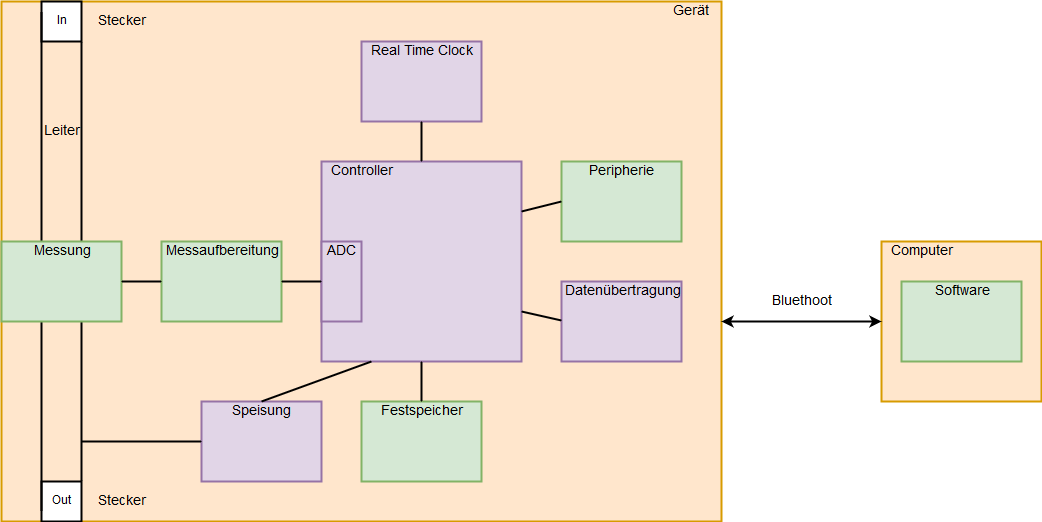
\includegraphics[scale=0.45]{P3T7-Blockdiagramm.png}
\\
\\
Die mit grün gekennzeichneten Felder werden selber designet während, die violett eingefärbten Felder direkt eingekauft werden.\\
Der orange Rahmen stellt das Gehäuse des Gerätes dar, die weissen Felder stehen für den jeweiligen Pol des Steckers.

\newpage
\section{Produkt Anforderungen}
\begin{itemize}
\item Das Messgerät muss mit den SEV 1011 Steckverbinder kompatibel sein.
\item Durch ein Kunststoffgehäuse muss die Schutzart IP 20 gewährleistet werden.
\item Wenn das Gerät nicht der Schutzklasse 2 entspricht muss eine Potenzialtrennung vorhanden sein.
\item Die Messung muss für Û=325V und Î=15A (Netzspannung) ausgelegt sein.
\item Harmonische Schwingungen bis 5kHz müssen detektiert werden.
\item Der Log Intervall der Leistung muss$\leq \ $10s sein.

\item Firmware für die Signalwandlung, Leistungsberechnung, Datenspeicherung und den Transfer zum Empfangsgerät.
\item Es muss eine Software mitgeliefert werden, welche den Empfang und die Darstellung des Leistungsgerätes sicherstellt. 

\item Die Daten werden über Bluetooth an eine Computer-Applikation gesendet, welcher als Empfänger dient. 
\end{itemize}


\section{Technische Daten}

 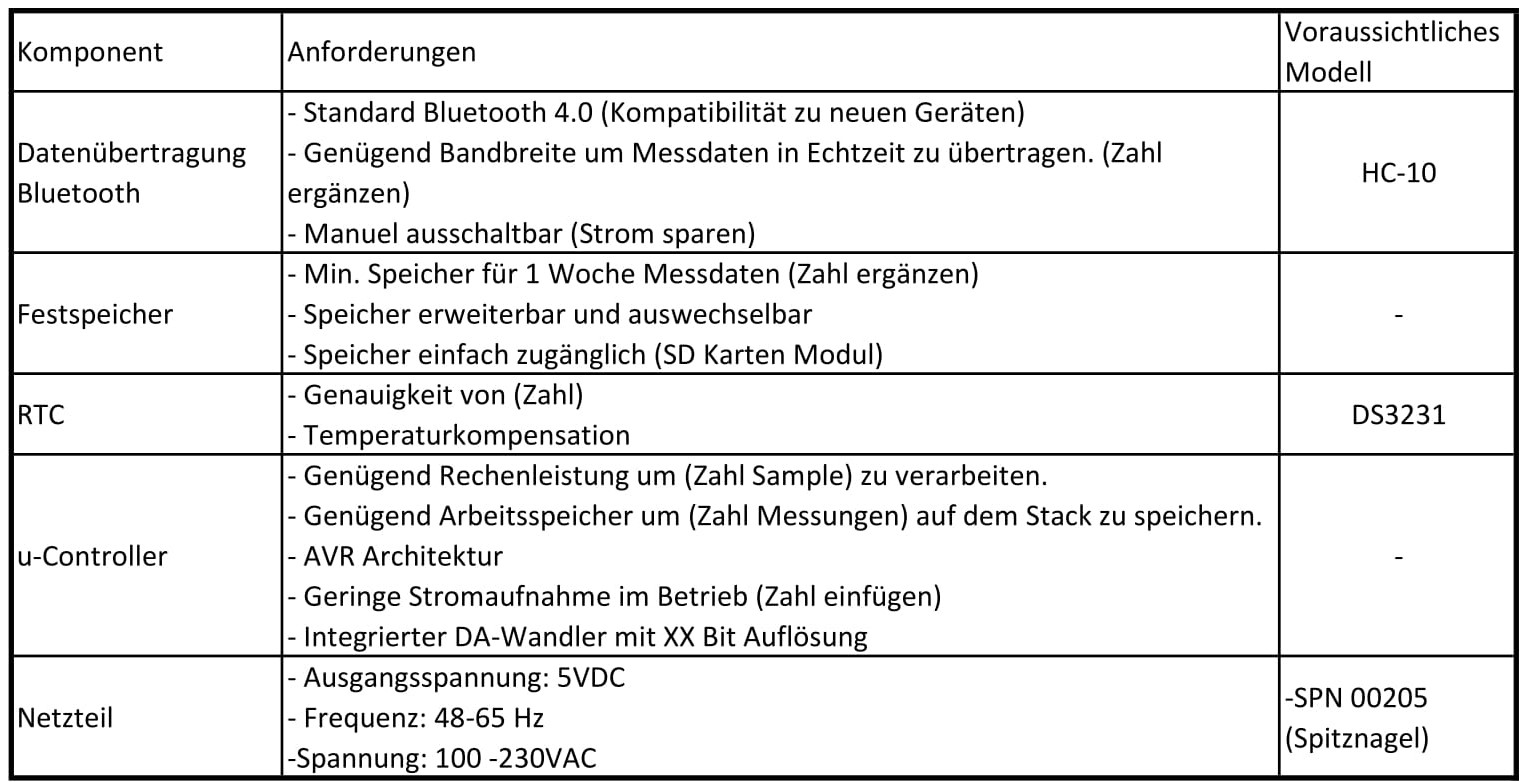
\includegraphics[scale=0.45]{Komp-1.jpg}

\subsection{Messung}
Für die Spannungsmessung wird ein Spannungteiler mit dem Verhältnis 100 zu 0,75 benötigt. Die Spannung muss im Bereich von 0-5V liegen. Die Spannung über dem kleineren Widerstand ($\pm 2,42V$) über einen Addierer in den gewünschten Bereich verschoben.\\
Für die Strommessung wird ein Messshunt verwendet.
\subsection{Messaufbereitung}
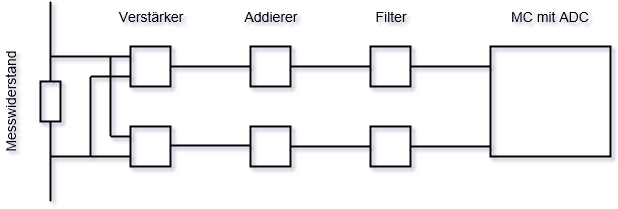
\includegraphics[scale=0.9]{Block-Messung.png}\\
Die Aufbereitung des Signals soll in drei Stufen erfolgen. In einem ersten Schritt soll das Signal mithilfe einer Instrument-Verstärkerschaltung auf maximal +/- 2.5V verstärkt werden. Danach wird im Addierer das Signal auf das Potential des Controllers gehoben. Dies wird mit einer Einkoppelung realisiert. Im Filter werden noch die unerwünschten Oberwellen oberhalb von 5kHz herausgefiltert. Da der Controller voraussichtlich eine 10 Bit Auflösung haben wird, wird der Messberiech in zwei Bereiche aufgeteilt, die entsprechend auf ihren Messbereich angepasst werden.

\subsection{Datenübertragung}
Für die Drahtlosübertragung werden wir ein Bluetoothmodul verwenden. Dafür bevorzugen wir im Moment das \glqq Seriell Protokoll Profil\grqq(SPP). Mit diesem Profil wird über Bluetooth eine serielle RS232 Schnittstelle aufgebaut, mit welcher wir mit maximal 115'200 bps erreichen können.\\ 
Wenn wir somit die Daten übertragen, können wir bei einer maximalen Übertragungsdauer von zehn Sekunden maximal 20 Bit alle 10 Sekunden abspeichern. Zudem haben wir für die Lifeübertragung 45 Bit Daten alle 0,5 Millisekunden zu Verfügung. Dies sollte für unsere Anforderungen ausreichen.


\subsection{Datenspeicherung}
Um Energiespitzen mit einer harmonischen Frequenz von 5kHz messen zu können, addieren wir den Energieverbrauch von 0.1ms über 10s auf und speichern diesen Wert im Festspeicher. Es sind immer die Daten der letzten sieben Tagen im Festspeicher vorhanden, welche über die Drahtlosschnittstelle ausgelesen werden können.

\subsection{Soft- und Firmware}
Zur Visualisierung und Auswertung der Messdaten wird eine Software auf der Basis von Java entwickelt. Diese Software erlaubt es, sich mit dem Gerät zu Verbinden und die gespeicherten Messdaten abzurufen. Ausserdem erlaubt sie die Echtzeit-Visualisierung der Leistungsmessung. 
\\
Die Firmware des u-Controllers managt die Speicherung und den Austausch der Messdaten. Die Rohdaten der Messung werden im Stack zwischengespeichert und alle (Zahl ergänzen) gemittelt. Dieser Mittelwert wird zusammen mit einem Zeitstämpel im Festspeicher abgelegt. Beim Datenaustausch mit der PC-Software regelt die Firmware den Lese- und Schreibzugriff auf den Festspeicher und stellt die synchronität der Daten sicher. 


\end{document}